\section {Opis baze podataka}
\label{sec:database}

Putem dijagrama klasa na slici \ref{fig:dijagram_klasa} je predstavljena baza.

U bazi su predstavljeni podaci podeljeni u 4 grupe podataka:
\begin{itemize}
    \item Podaci o osoblju i kandidatu
    \item Podaci o ispitu
    \item Podaci o nastavi
    \item Ostali podaci
\end{itemize}


\subsection{Podaci o osoblju i kandidatu}

\textbf{\large Osoba}
\vspace{0.3cm}

Klasa \textit{Osoba} predstavlja osnovne informacije o korisnicima našeg sistema. 
Iz ovog tipa entiteta primenom specijalizacije izvodimo 2 nova tipa entiteta: Osoblje i Kandidat.

Atributi:
\begin{itemize}
    \item id - jedinstveni identifikator korisnika (PK, automatski generisan)
    \item lozinka 
    \item ime
    \item prezime
    \item jmbg
    \item pol
    \item telefon
\end{itemize}

\textbf{\large Osoblje}
\vspace{0.3cm}

Klasa \textit{Osoblje} predstavlja zaposlene osobe u našem sistemu.
Iz ovog tipa entiteta primenom specijalizacije izvodimo 6 novih tipova entiteta: 
Predavač, Instruktor, Nadležni za zaposlene, Računovođa, Administrativni radnik i Administrator sistema.

Atributi:
\begin{itemize}
    \item brojRačuna
    \item visinaPlate
    \item datumZaposlenja
\end{itemize}

\textbf{\large Kandidat}
\vspace{0.3cm}

Klasa \textit{Kandidat} predstavlja jednog kandidata koji je upisan u auto školu.

Atributi:
\begin{itemize}
    \item datumRođenja
    \item datumUpisa
    \item idInstruktora - instruktor koji drži kandidatu časove vožnje (SK koji referiše na Instruktor)
    \item idGrupe - grupa u koju je kandidat raspoređen (SK koji referiše na Grupa)
\end{itemize}


\textbf{\large Instruktor}
\vspace{0.3cm}

Klasa \textit{Instruktor} predstavlja zaposlenog koji je zadužen da drži časove praktične nastave.

Atributi:
\begin{itemize}
    \item idVozila - vozilo koje je dodeljeno instruktoru (SK koji referiše na Vozilo)
    \item ocena - trenutna ocena za instruktora na osnovu rezultata ankete
\end{itemize}

\subsection{Podaci o nastavi}

\textbf{\large Nastava}
\vspace{0.3cm}

Klasa \textit{Nastava} predstavlja osnovne informacije o nastavi u auto školi. Iz ovog tipa entiteta primenom specijalizacije izvodimo 2 nova tipa entiteta: Praktična nastava i Teorijska nastava.

Atributi:
\begin{itemize}
    \item id - jedinstveni identifikator ispita (PK, automatski generisan)
    \item datumOdržavanja
    \item vremeOdržavanja
\end{itemize}

\textbf{\large Teorijska nastava}
\vspace{0.3cm}

Klasa \textit{Teorijska nastava} predstavlja osnovne informacije vezano za teorijsku nastavu.

Atributi:
\begin{itemize}
    \item idPredavača (SK koji referiše na Predavač)
    \item brojSale
    \item idGrupe (SK koji referiše na Grupa)
\end{itemize}

\textbf{\large Praktična nastava}
\vspace{0.3cm}

Klasa \textit{Praktična nastava} predstavlja osnovne informacije vezano za praktičnu nastavu.

Atributi:
\begin{itemize}
    \item idInstruktora (SK koji referiše na Instruktor)
    \item brojRute
    \item idKandidata (SK koji referiše na Kandidat)
    \item nocnaVoznja
    \item idVozila (SK koji referiše na Vozilo)
\end{itemize}


\subsection{Podaci o ispitu}

\textbf{\large Ispit}
\vspace{0.3cm}

Klasa \textit{Ispit} predstavlja osnovne informacije o ispitu. 
Iz ovog tipa entiteta primenom specijalizacije izvodimo 2 nova tipa entiteta: Praktični ispit i Teorijski ispit.
Klasa \textit{Teorijski ispit} predstavlja osnovne informacije vezano za polaganje teorijskog ispita.
Klasa \textit{Praktični ispi} predstavlja osnovne informacije vezano za polaganje praktičnog ispita.

Atributi:
\begin{itemize}
    \item id - jedinstveni identifikator ispita (PK, automatski generisan)
    \item datumPolaganja 
    \item vremePolaganja
    \item idKandidata - koji polaže praktični/teorijski ispit(SK koji referiše na Kandidat)
    \item statusPolaganja
    \item brojPoena 
\end{itemize}






\subsection{Ostali podaci}

\textbf{\large Vozilo}
\vspace{0.3cm}

Klasa \textit{Vozilo} predstavlja osnovne informacije o stanju vozila

Atributi:
\begin{itemize}
    \item id - jedinstveni identifikator ispita (PK, automatski generisan)
    \item registracioniBroj
    \item model
    \item datumRegistracije
    \item pređeniKm
\end{itemize}

\textbf{\large Anketa}
\vspace{0.3cm}

Klasa \textit{Anketa} predstavlja jednu anketu koju kandidat popunjava unoseći utiske o instruktoru.

Atributi:
\begin{itemize}
    \item id (PK, automatski generisan)
    \item idKandidata - kandidat koji popunjava anketu (SK koji referiše na Kandidat)
    \item ocena - ocena koju daje instruktoru
\end{itemize}

\textbf{\large Grupa}
\vspace{0.3cm}

Klasa \textit{Grupa} predstavlja osnovne informacije o jednoj polaznoj grupi kandidata koji pohađaju teorijsku nastavu.

Atributi:
\begin{itemize}
    \item id (PK, automatski generisan)
    \item brojKandidata 
    \item idPredavača - predavač koji je dodeljen grupi (SK koji referiše na Predavač)
\end{itemize}

Klasa \textit{Uplata} predstavlja podatke o jednoj uplati kandidata, u određenom iznosu, po cenovniku usluga auto škole.

Atributi:
\begin{itemize}
    \item id (PK, automatski generisan)
    \item idRačunovođe - računovođa koji evidentira uplatu (SK koji referiše na Računovođa)
    \item idKandidata - kandidat koji vrši uplatu u određenom iznosu (SK koji referiše na Kandidat)
    \item iznos
    
\end{itemize}




\begin{figure}[H]
    \begin{center}
        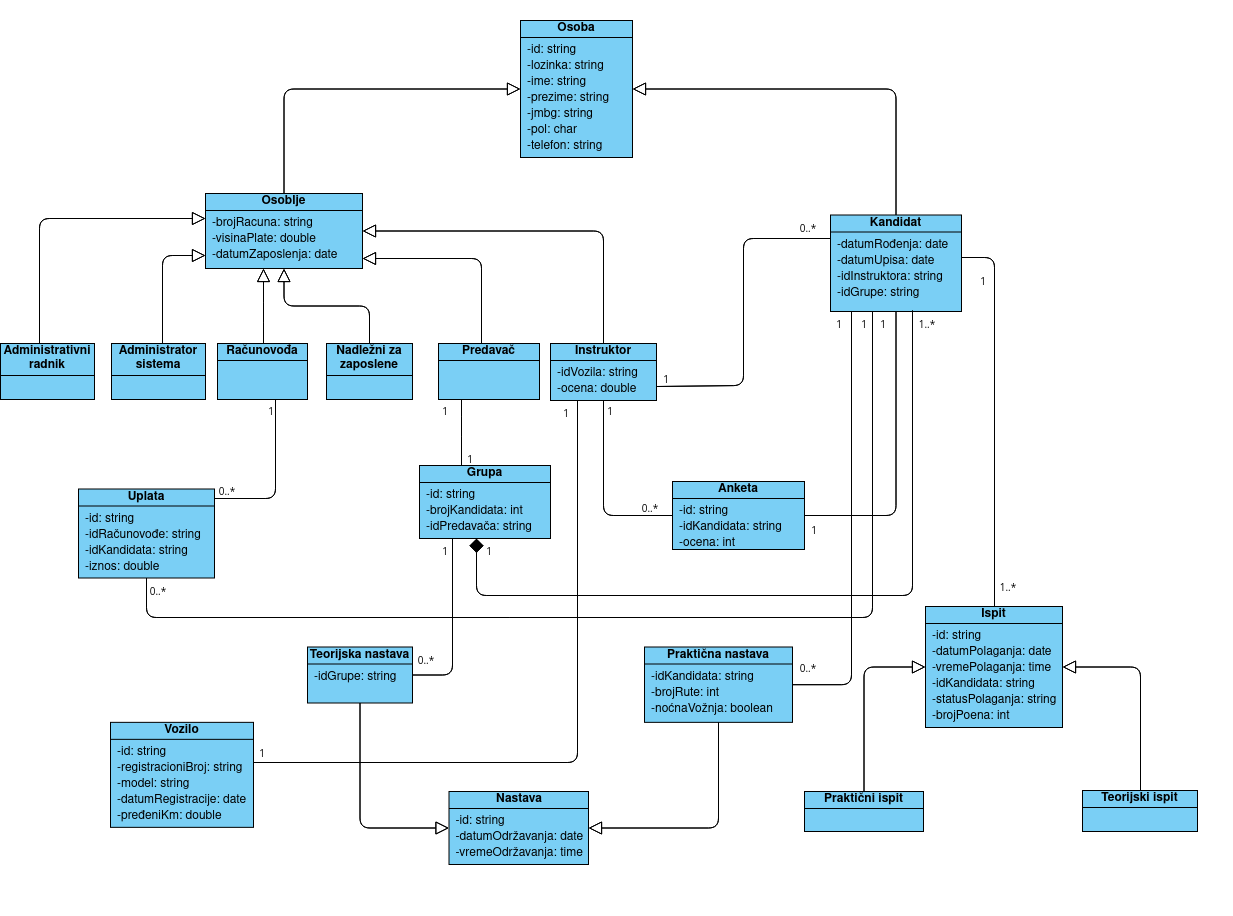
\includegraphics[width=\textwidth, height=170mm]{Diagrams/dijagram_klasa.png}
        \caption {Dijagram klasa baze podataka}
        \label{fig:dijagram_klasa}
    \end{center}
\end{figure}
